\documentclass{article}

\usepackage[margin=0.5in]{geometry}
\usepackage{enumitem}
\usepackage{amsmath}
\usepackage{bbm}
\usepackage{amssymb}
\usepackage{cancel}
\usepackage{todonotes}
\usepackage{listings}
\usepackage{grffile}
\usepackage{graphicx}
\usepackage{array}
\usepackage{graphicx}
\usepackage{subcaption}
\usepackage{mwe}
\usepackage{tabularx}

\DeclareMathOperator{\EX}{\mathbb{E}}% expected value
\DeclareMathOperator{\VAR}{\mathbb{V}}% expected value
\DeclareMathOperator*{\argmin}{arg\,min}
\DeclareMathOperator*{\argmax}{arg\,max}

\newcommand{\bs}{\boldsymbol}
\newcommand{\tb}{\textbf}
\newcommand{\pc}[2]{p(#1 \mid #2)}
\newcommand{\mc}[1]{\mathcal{#1}}
\newcommand{\half}{\frac{1}{2}}
\newcommand{\C}{(2\pi)^{-d}\psi^{-\frac{d}{2}}|\Upsilon|}
\newcommand{\D}{exp\left(-\half\tb{x}^T\psi^{-1}\tb{x}\right)}
\newcommand{\inv}[1]{#1^{-1}}
\newcommand{\sumlim}[3]{\sum\limits_{#1 = #2}^{#3}}
\newcommand{\suml}[1]{\sum\limits_{#1}}
\newcommand{\prodlim}[3]{\prod\limits_{#1 = #2}^{#3}}
\newcommand{\prodl}[1]{\prod\limits_{#1}}
\newcommand{\ub}{\underbrace}
\newcommand{\intlim}[2]{\int\limits_{#1}^{#2}}
\newcommand{\diff}[1]{\frac{d}{d#1}}
\newcommand{\prl}{\partial}
\newcommand{\ol}{\overline}
\newcommand{\argminl}[1]{\argmin\limits_{#1}^{}}
\newcommand{\argmaxl}[1]{\argmax\limits_{#1}^{}}
\newcommand{\mbb}{\mathbb}

\renewcommand{\bs}{\boldsymbol}

\allowdisplaybreaks

\title{Gaussian RGG}
\author{}
\date{}

\begin{document}

\maketitle

\section{Work}
We are given a graph $\mc{G}$ with $N$ and $E$ edges. Let $X = \{X_i\}_{i \in [N]}$ be the set of embeddings for the vertices we are trying to infer from the data, modelled iid by a prior multivariate Gaussian

\begin{equation*}
    X_i \sim \mc{N}(\bs{0}, \mc{I}_n)
\end{equation*}

\noindent
where $n$ is the number of dimensions of the space in which the embeddings lie. The existence of an edge between two vertices will be randomly determined, based on the distance between their corresponding embeddings. Please note that the mean of the distribution is irrelevant when working with a single distribution, since we could just shift all the points such that the mean bocomes $0$ and the graph will remain the same.\\

\noindent
Let

\begin{equation*}
    X_{ij} \sim \text{Bernoulli}(e^{-d_{ij}^2})
\end{equation*}

\noindent
be a random variable representing the existence of an edge between the $i^\text{th}$ and $j^\text{th}$ vertex, where $d_{ij}$ is the Euclidean distance between their corresponding embeddings, $X_i$ and $X_j$. \\

\noindent
We are looking to approximate the posterior distribution

\begin{equation*}
    P(X \mid \mc{G}) \propto P(\mc{G} \mid X) P(X)
\end{equation*}

\noindent
by a multivariate Gaussian with spherical covariance matrix determined by parameter $\sigma$

\begin{equation*}
    P(X \mid \mc{G}) \approx q(X) = \mc{N}(X;\, 0,\, \sigma^2 \mc{I}_n)
\end{equation*}

\noindent
Therefore, we look to maximise the free energy as a function of $\sigma$ for the best approximation.

\begin{equation}
    \mc{F}(\sigma) = \left< log P(\mc{G} \mid X)\right>_{q(X)} - \text{KL}\left(P(X) || q(X))\right)
\end{equation}

\noindent
The first term becomes

\begin{align*}
    \left<logP(\mc{G}\mid X)\right>_{q(X)} &= \int\limits_{[\mbb{R}^n]^N} dX\, q(X)\, logP(\mc{G}\mid X) \\
    &= \int\limits_{[\mbb{R}^n]^N} dX\, q(X)\, \sum\limits_{i < j} P(X_{ij} \mid X_i, X_j) \\
    &= \sum\limits_{i < j}\int\limits_{[\mbb{R}^n]^2} dX_i dX_j\, q(X_i, X_j)\,  logP(X_{ij} \mid X_i, X_j) \\
    &= \sum\limits_{i < j}\int\limits_{[\mbb{R}^n]^2} dX_i dX_j\, q(X_i, X_j)\,  log\left[(e^{-d_{ij}^2})^{X_{ij}}(1 - e^{-d_{ij}^2})^{1 - X_{ij}}\right] \\
    &= \sum\limits_{i < j}\int\limits_{\mbb{R}^n} dX_i \intlim{0}{\infty} du\, log\left[(e^{-u})^{X_{ij}}(1 - e^{-u})^{1 - X_{ij}}\right] \int\limits_{\mc{X} = \{X_j \in \mbb{R}^n : d(X_i, X_j)^2 = u\}} dX_j\, q(X_i, X_j)\,   \\
    &= \sum\limits_{i < j}\intlim{0}{\infty} du\, log\left[(e^{-u})^{X_{ij}}(1 - e^{-u})^{1 - X_{ij}}\right] \ub{\int\limits_{\mbb{R}^n} dX_i \int\limits_{\mc{X} = \{X_j \in \mbb{R}^n : d(X_i, X_j)^2 = u\}} dX_j\, q(X_i, X_j)}_{q(u)}\,   \\
\end{align*}

where $q(u)$ is the pdf of the squared Euclidean distance between two independent points modelled by a Gaussian distribution. \\

\noindent
The squared distance can be written as $(X_1 - X_2)^T(X_1 - X_2)$, where

\begin{align*}
    X_1 &\sim \mc{N}(0, \tau_1^2\mc{I}_n)\\
    X_2 &\sim \mc{N}(0, \tau_2^2\mc{I}_n)
\end{align*}

\noindent
so $U \sim Y^TY$, where $Y \sim \mc{N}(0, \ub{(\tau_1^2 + \tau_2^2)}_{\tau^2}\mc{I}_n)$ \\

\noindent
Assuming that $n$ is even, we work out that

\begin{equation}
    q(u) = \frac{(2\tau^2)^{-m}}{(m - 1)!} u^{m - 1}e^{-\frac{u}{2\tau^2}},\quad\text{where}\,\, m = \frac{n}{2} \in \mbb{N}
\end{equation}

\noindent
In the expected log likelihood, the covariances of the embeddings have the same value, $\sigma^2$, so our $q(u)$ becomse

\begin{equation}
    q(u) = \frac{(2 \times 2\sigma^2)^{-m}}{(m - 1)!} u^{m - 1}e^{-\frac{u}{2 \times 2\sigma^2}},\quad\text{where}\,\, m = \frac{n}{2} \in \mbb{N}
\end{equation}

\begin{figure}[ht]
    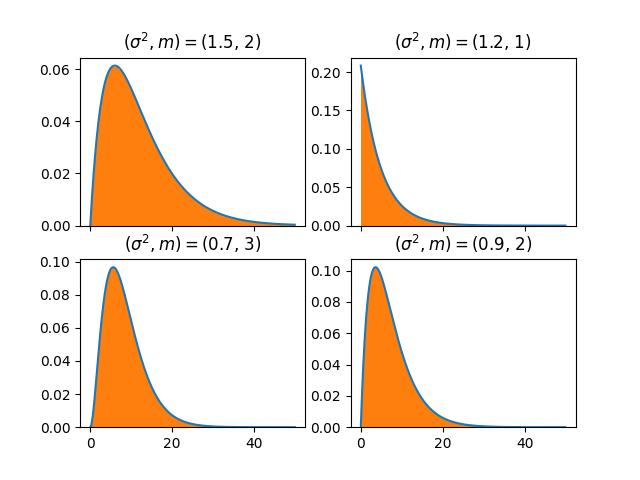
\includegraphics{sq_distance_pdf.png}
    \caption{The blue line is the pdf of the squared distance between two random normals, as calculated at (3) and the orange plot is a histogram of the squared distance between $10^7$ samples of two normally distributed points.}
\end{figure}

\noindent
Using this result, we can calculate the expected number of edges in a graph, for N embeddings generated using the covariance matrix $\sigma^2\mc{I}_n$.

\begin{align*}
    \EX[\text{\#edges}] &= \begin{pmatrix} N \\ 2 \end{pmatrix}\EX[X_{12}] \\
        &= \begin{pmatrix} N \\ 2 \end{pmatrix} \intlim{0}{\infty}du\, e^{-u} q(u) \\
        &= \begin{pmatrix} N \\ 2 \end{pmatrix} \intlim{0}{\infty}du\, e^{-u} \frac{(4\sigma^2)^{-m}}{(m - 1)!} u^{m - 1}e^{-\frac{u}{4\sigma^2}} \\
            &= \begin{pmatrix} N \\ 2 \end{pmatrix} \frac{1}{(1 + 4\sigma^2)^m} \\
\end{align*}

\noindent
Going back to the expected log likelihood, we have

\begin{align*}
    \left<logP(\mc{G}\mid X)\right>_{q(X)} &=\sum\limits_{i < j}\intlim{0}{\infty} du\, log\left[(e^{-u})^{X_{ij}}(1 - e^{-u})^{1 - X_{ij}}\right] q(u) \\
    &= E \intlim{0}{\infty} du\, log(e^{-u})q(u) + \left(\begin{pmatrix} N \\ 2 \end{pmatrix} - E\right)\intlim{0}{\infty} du\, log(1 - e^{-u})q(u)
\end{align*}

\noindent
where $E$ is the number of edges in the given graph. The first integral can be calculated \\


\begin{align*}
    \intlim{0}{\infty} du\, log(e^{-u})q(u) &= \intlim{0}{\infty} du\, -u \frac{(4\sigma^2)^{-m}}{(m - 1)!} u^{m - 1}e^{-\frac{u}{4\sigma^2}} \\
    &= -\intlim{0}{\infty} du\, \frac{(4\sigma^2)^{-m}}{(m - 1)!} u^{m}e^{-\frac{u}{4\sigma^2}} \\
    &= -\frac{1}{(m - 1)!}\intlim{0}{\infty} du\, \left(\frac{u}{4\sigma^2}\right)^{m} e^{-\frac{u}{4\sigma^2}} \\
    &= -\frac{1}{(m - 1)!} (4\sigma^2)\Gamma(m + 1) \\
    &= -4m\sigma^2 \\
\end{align*}

\noindent
For m = 2, for a set of sigmas, we calculate the expected number of edges in our graph and use that to optimise for sigma in our free energy. I said that there is some relationship between the original sigma and the recovered one, but, plotting for a larger sigma set, it looks like there is not a clear one. My hypothesis is that the approximate distribution, with its spherical covariance is too strong of an assumption and that is why it cannot recover the parameter. \\

\noindent
In the call I said that m does not matter, since, if we pick another m, we can just choose a different $\sigma$, making the distribution amount to the same thing. This is false. It would work only for the expected number of edges, not the pdf itself.


\begin{figure}[ht]
    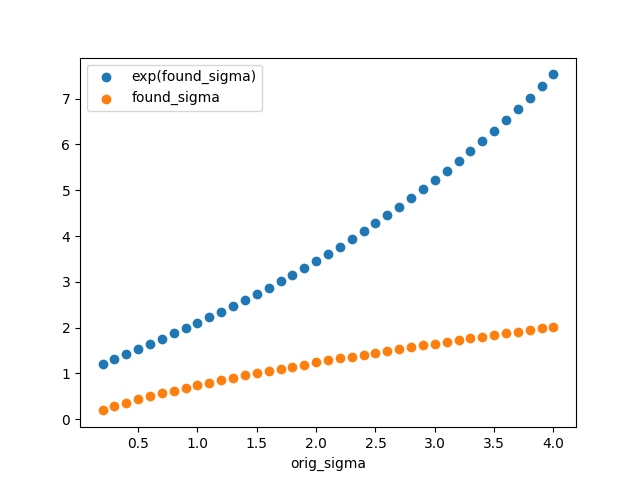
\includegraphics{orig_sigma_vs_found_sigma.png}
\end{figure}

\end{document}
